\documentclass{article}

\usepackage[final]{style}
\usepackage[utf8]{inputenc} % allow utf-8 input
\usepackage[T1]{fontenc}    % use 8-bit T1 fonts
\usepackage{hyperref}       % hyperlinks
\usepackage{url}            % simple URL typesetting
\usepackage{booktabs}       % professional-quality tables
\usepackage{amsfonts}       % blackboard math symbols
\usepackage{nicefrac}       % compact symbols for 1/2, etc.
\usepackage{microtype}      % microtypography
\usepackage{verbatim}
\usepackage{graphicx}       % for figures


\title{CS 131 Lecture 1: Course introduction}

\author{
  Olivier Moindrot \\
  Department of Computer Science\\
  Stanford University\\
  Stanford, CA 94305 \\
  \texttt{olivierm@stanford.edu} \\
}

\begin{document}

\maketitle


\section{What is computer vision?}
% - definition
% - 50 year old field
% - how is it used?
% - interdisciplinary
% - it is hard (why?)
% - what is vision?
\subsection{Definition}
\paragraph{Two definitions of computer vision}
Computer vision can be defined as \textit{a scientific field that extracts information out of digital images}. The type of information gained from an image can vary from identification, space measurements for navigation, or augmented reality applications.

Another way to define computer vision is through its applications. Computer vision is \textit{building algorithms that can understand the content of images and use it for other applications}. We will see in more details in section \ref{applications} the different domains where computer vision is applied.

\paragraph{A bit of history}
The origins of computer vision go back to an MIT undergraduate summer project in 1966 \cite{papert1966summer}. It was believed at the time that computer vision could be solved in one summer, but we now have a 50-year old scientific field which is still far from being solved.

\begin{figure}[h]
\begin{center}
\centerline{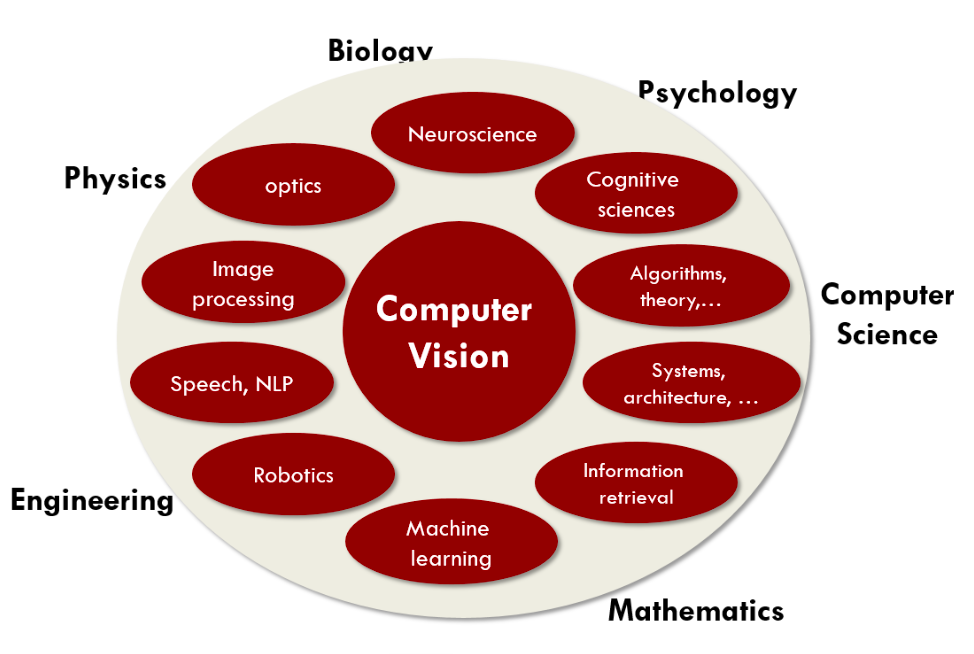
\includegraphics[width=0.8\columnwidth]{fields.png}}
\caption{Computer vision at the intersection of multiple scientific fields}
\label{fields}
\end{center}
\end{figure} 

\subsection{An interdisciplinary field}

Computer vision brings together a large set of disciplines. Neuroscience can help computer vision by first understanding human vision, as we will see in section \ref{solving}. Computer vision can be seen as a part of computer science, and algorithm theory or machine learning are essential for developing computer vision algorithms.

We will show in this class how all the fields in figure \ref{fields} are connected, and how computer vision draws inspiration and techniques from them.

\subsection{A hard problem}

Computer vision has not been solved in 50 years, and is still a very hard problem. It's something that we humans do unconsciously but that is genuinely hard for computers.

\paragraph{Poetry harder than chess}
The IBM supercomputer Deep Blue defeated for the first time the world chess champion Garry Kasparov in 1997. Today we still struggle to create algorithms that output well formed sentences, let alone poems.
The gap between these two domains show that what humans call \textit{intelligence} is often not a good criteria to assess the difficulty of a computer task. Deep Blue won through brute force search among millions of possibilities and was not more \textit{intelligent} than Kasparov.

\paragraph{Vision harder than 3D modeling}
It is today easier to create a 3D model of an object up to millimeter precision than to build an algorithm that recognizes chairs. Object recognition is still a very difficult problem, although we are approaching human accuracy.

\paragraph{Why is it so hard?}
Computer vision is hard because there is a huge gap between pixels and meaning. What the computer sees in a $200 \times 200$ RGB image is a set of $120,000$ values. The road from these numbers to meaningful information is very difficult. Arguably, the human brain's visual cortex solves a problem as difficult: understanding images that are projected on our retina and converted to neuron signals. The next section will show how studying the brain can help computer vision.


\section{Understanding human vision} \label{solving}
% what is vision
% simulating the brain
% humans visual system very good
% but can be fooled
% context is powerful
% conclusion: we didn't imitate birds to fly planes, but studying them made us understood aerodynamics
A first idea to solve computer vision is to understand how human vision works, and transfer this knowledge to computers.

\subsection{Definition of vision}
Be it a computer or an animal, vision comes down to two components.

First, a \textbf{sensing device} captures as much details from an image as possible. The eye will capture light coming through the iris and project it to the retina, where specialized cells will transmit information to the brain through neurons. A camera captures images in a similar way and transmit pixels to the computer. In this part, cameras are better than humans as they can see infrared, see farther away or with more precision.

Second, the \textbf{interpreting device} has to process the information and extract meaning from it. The human brain solves this in multiple steps in different regions of the brain. Computer vision still lags behind human performance in this domain.

\subsection{The human visual system}

In 1962, Hubel \& Wiesel \cite{hubel} tried to understand the visual system of a cat by recording neurons while showing a cat bright lines. They found that some specialized neurons fired only when the line was in a particular spot on the retina or if it had a certain orientation.
\footnote{More information in \href{http://knowingneurons.com/2014/10/29/hubel-and-wiesel-the-neural-basis-of-visual-perception/}{this blog post}}

Their research led to the beginning of a scientific journey to understand the human visual system, which is still active today.

They were awarded the Nobel Prize in Physiology and Medecine in 1981 for their work. After the announcement, Dr. Hubel said:
\begin{quote}
There has been a myth that the brain cannot understand itself.  It is compared to a man trying to lift himself by his own bootstraps.  We feel that is nonsense.  The brain can be studied just as the kidney can.
\end{quote}


\subsection{How good is the human visual system?}
\paragraph{Speed}
The human visual system is very efficient. As recognizing threats and reacting to them quickly was paramount to survival, evolution perfected the visual system of mammals for millions of years.

The speed of the human visual system has been measured \cite{speed} to around 150ms to recognize an animal from a normal nature scene. Figure \ref{fig:speed} shows how the brain response to images of animals and non-animals diverge after around 150ms.

\begin{figure}[h]
\begin{center}
\centerline{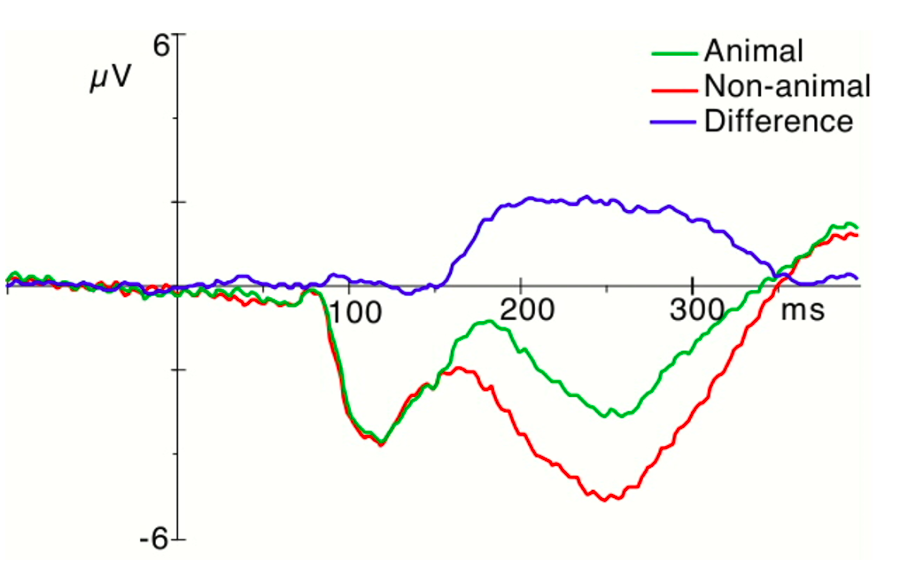
\includegraphics[width=0.8\columnwidth]{speed.png}}
\caption{Difference between animal and non-animal response. From \cite{speed}}
\label{fig:speed}
\end{center}
\end{figure} 


\paragraph{Fooling humans}
However, this speed is obtained at the price of some drawbacks. Changing small irrelevant parts of an image such as water reflection or background can go unnoticed because the human brain focuses on the important parts of an image \cite{failure}.

If the signal is very close to the background, it can be difficult to detect and segment the relevant part of the image.

\paragraph{Context}
Humans use context all the time to infer clues about images. Previous knowledge is one of the most difficult tool to incorporate into computer vision. Humans use context to know where to focus on an image, to know what to expect at certain positions. Context also helps the brain to compensate for colors in shadows.

However, context can be used to fool the human brain.

\subsection{Lessons from nature}
Imitating birds did not lead humans to planes. Plainly copying nature is not the best way or the most efficient way to learn how to fly. But studying birds made us understand aerodynamics, and understanding concepts like lift allowed us to build planes.

The same might be true with intelligence. Even though it is not possible with today's technology, simulating a full human brain to create intelligence might not be the best way to get there. However, neuroscientists hope to get insights at what may be the concepts behind vision, language and other forms of intelligence.

% -------------------
\section{Extracting information from images}

We can divide the information gained from images in computer vision in two categories: measurements and semantic information.

\subsection{Vision as a measurement device}
Robots navigating in an unknown location need to be able to scan their surroundings to compute the best path. Using computer vision, we can measure the space around a robot and create a map of its environment.

Stereo cameras give depth information, like our two eyes, through triangulation. Stereo vision is a big field of computer vision and there is a lot of research seeking to deduce a precise depth map given stereo images.

If we increase the number of viewpoints to cover all the sides of an object, we can create a 3D surface representing the object \cite{multipleview}.

An even more challenging idea might be to reconstruct the 3D model of a monument through all the results of a google image search for this monument \cite{multicommunity}.

There is also research in grasping, where computer vision can help understand the 3D geometry of an object to help a robot grasp it. Through the camera of the robot, we could recognize and find the handle of the object and infer its shape, to then enable the robot to find a good grasping position \cite{grasping}.


\subsection{A source of semantic information}

On top of measurement informations, an image contains a very dense amount of \textit{semantic information}. We can label objects in an image, label the whole scene, recognize people, recognize actions, gestures, faces.

Medical images also contain a lot of semantic information. Computer vision can be helpful for a diagnosis based on images of skin cells for instance, to decide if they are cancerous or not.



% -------------------
\section{Applications of computer vision} \label{applications}
% cameras are everywhere
% special effects
% 3D urban modeling
% scene recognition
% face detection
% OCR
% self-driving cars
% automatic checkout (Amazon)
% Kinect
% AR
% VR
% Space exploration

Cameras are everywhere and the number of images uploaded on internet is growing exponentially. We have images on Instagram, videos on YouTube, feeds of security cameras, medical and scientific images... Computer vision is essential because we need to sort through these images and enable computers to understand their content. Here is a non exhaustive list of applications of computer vision.


\paragraph{Special effects}
Shape and motion capture are new techniques used in movies like Avatar to animate digital characters by recording the movements played by a human actor. In order to do that, we have to find the exact positions of markers on the actor's face in a 3D space, and then recreate them on the digital avatar.

\paragraph{3D urban modeling}
Taking pictures with a drone over a city can be used to render a 3D model of the city. Computer vision is used to combine all the photos into a single 3D model.

\paragraph{Scene recognition}
It is possible to recognize the location where a photo was taken. For instance, a photo of a landmark can be compared to billions of photos on google to find the best matches. We can then identify the best match and deduce the location of the photo.

\paragraph{Face detection}
Face detection has been used for multiple years in cameras to take better pictures and focus on the faces. Smile detection can allow a camera to take pictures automatically when the subject is smiling. Face recognition is more difficult than face detection, but with the scale of today's data, companies like Facebook are able to get very good performance. Finally, we can also use computer vision for biometrics, using unique iris pattern recognition or fingerprints.

\paragraph{Optical Character Recognition}
One of the oldest successful applications of computer vision is to recognize characters and numbers. This can be used to read zipcodes, or license plates.

\paragraph{Mobile visual search}
With computer vision, we can do a search on Google using an image as the query.

\paragraph{Self-driving cars}
Autonomous driving is one of the hottest applications of computer vision. Companies like Tesla, Google or General Motors compete to be the first to build a fully autonomous car.

\paragraph{Automatic checkout}
Amazon Go is a new kind of store that has no checkout. With computer vision, algorithms detect exactly which products you take and they charge you as you walk out of the store \footnote{see their video \href{https://www.amazon.com/b?node=16008589011}{here}}.

\paragraph{Vision-based interaction}
Microsoft's Kinect captures movement in real time and allows players to interact directly with a game through moves.

\paragraph{Augmented Reality}
AR is also a very hot field right now, and multiple companies are competing to provide the best mobile AR platform. Apple released ARKit in June and has already impressive applications \footnote{check out the different \href{http://www.madewitharkit.com}{apps}}.

\paragraph{Virtual Reality}
VR is using similar computer vision techniques as AR. The algorithm needs to know the position of a user, and the positions of all the objects around.





% References
\small
\bibliographystyle{plain}
\bibliography{bibliography}
\end{document}
